\section*{Exercice 1 -- Représentation du coût temporel des tris}


\ifprof
\else

\begin{obj}
Représenter pour chacun des tris les courbes indiquant le temps d'exécution en fonction du nombre d'éléments à trier.
\end{obj}
On donne la bibliothèque de tri \texttt{tris.py} dans laquelle différents tris ont été implémentés.
On dispose ainsi des fonctions : 
\begin{itemize}
\item \texttt{tri\_insertion};
\item \texttt{tri\_rapide};
\item \texttt{tri\_fusion}.
\end{itemize}
On dispose aussi de la méthode \texttt{sort} disponible en Python.

On utilisera de plus le module \texttt{time} de la bibliothèque \texttt{time} pour créer un chronomètre et le module \texttt{randint} de la bibliothèque \texttt{random}.

Pour augmenter la limite de récursivité de Python, on utilisera les instructions suivantes : \texttt{import sys} puis \texttt{sys.setrecursionlimit(100000)}.

\subparagraph{}
\textit{Tracer, dans chacun des 4 cas, le temps de tri d'une liste en fonction du nombre d'éléments de la liste. Le nombre d'éléments variera de $0$ à $1\, 000$ par pas de 100. Une liste de $n$ éléments sera composée de nombres choisis aléatoirement entre 0 et $n$. Ce réseau de courbes représentera le cas moyen.}

\subparagraph{}
\textit{Tracer, dans le cas des trois tris les plus rapides, le temps de tri d'une liste en fonction du nombre d'éléments de la liste. Le nombre d'éléments variera de $0$ à $20\, 000$. Une liste de $n$ éléments sera composée de nombres choisis aléatoirement entre 0 et $n$. Ce réseau de courbes représentera le cas moyen.}

\subparagraph{}
\textit{Conclure sur l'efficacité algorithme de chacun des tris dans le cas moyen.}

\subparagraph{}
\textit{Comparer les temps de tris de chacune des 4 méthodes sur une liste triée d'un million d'éléments. Que peut-on en conclure ?}


\fi


\ifprof
\begin{corrige}

\question\ 

\begin{python}
import sys
sys.path.insert(0, 'eleves')
import tris

import random as rd
import time
import matplotlib.pyplot as plt
import sys
sys.setrecursionlimit(1000000) # cette ligne permet de modifier le nombre
# de boucles récursives autorisées (normalement de 1000)

def question_1 () :
    longueur = [n for n in range(0,1001,100)]
    moyenne_insert = []
    moyenne_rapide = []
    moyenne_fusion = []
    moyenne_sort = []
    for n in longueur :
        # n = longueur des listes que l'on va trier
        temps_insert = []
        temps_rapide = []
        temps_fusion = []
        temps_sort = []
        for m in range(10) :
            # on va trier 10 listes et faire la moyenne des temps de calcul
            M = [rd.randint(0,n) for i in range(n)] # liste aléatoire de
                        # n éléments entre 0 et n
                        
            L = M.copy()            
            temps=time.time()
            tris.tri_insertion(L)
            temps = time.time() - temps
            temps_insert.append(temps)

            L = M.copy()
            temps=time.time()
            tris.tri_fusion(L,0,n-1)
            temps = time.time() - temps
            temps_fusion.append(temps)
            
            L = M.copy()
            temps=time.time()
            tris.tri_quicksort(L,0,n-1)
            temps = time.time() - temps
            temps_rapide.append(temps)
            
            L = M.copy()
            temps=time.time()
            L.sort()
            temps = time.time() - temps
            temps_sort.append(temps)
            
        moyenne_insert.append(sum(temps_insert)/m)
        moyenne_rapide.append(sum(temps_rapide)/m)
        moyenne_fusion.append(sum(temps_fusion)/m)
        moyenne_sort.append(sum(temps_sort)/m)

    plt.clf()
    plt.grid()
    plt.xlabel('taille de la liste')
    plt.ylabel('temps de tri en seconde')
    plt.plot(longueur,moyenne_insert,label='insertion')
    plt.plot(longueur,moyenne_rapide,label='rapide')
    plt.plot(longueur,moyenne_fusion,label='fusion')
    plt.plot(longueur,moyenne_sort,label='sort')
    plt.legend(loc='upper left')
    plt.savefig("question_1.png")
\end{python}


\begin{figure}[H]
\begin{center}
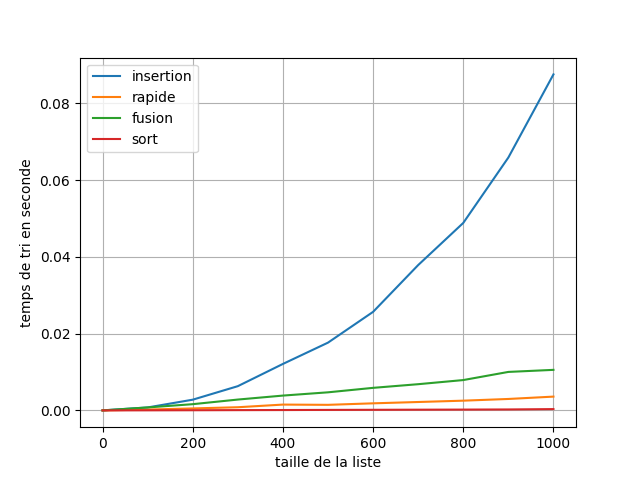
\includegraphics[scale=0.8]{programmes/question_1.png}
\caption{Temps de calcul des tris}
\end{center}
\end{figure}

\question\

\begin{python}
def question_2 () :
    # on commencera avec des listes de 10000 éléments, en allant
    # de 1000 en 1000, sinon le temps de calcul est trop long.
    longueur = [n for n in range(10000,20001,1000)]
    moyenne_rapide = []
    moyenne_fusion = []
    moyenne_sort = []
    for n in longueur :
        # n = longueur des listes que l'on va trier
        temps_insert = []
        temps_rapide = []
        temps_fusion = []
        temps_sort = []
        for m in range(10) :
            # on va trier 10 listes et faire la moyenne des temps de calcul
            M = [rd.randint(0,n) for i in range(n)] # liste aléatoire de
                        # n éléments entre 0 et n
                        

            L = M.copy()
            temps=time.time()
            tris.tri_fusion(L,0,n-1)
            temps = time.time() - temps
            temps_fusion.append(temps)
            
            L = M.copy()
            temps=time.time()
            tris.tri_quicksort(L,0,n-1)
            temps = time.time() - temps
            temps_rapide.append(temps)
            
            L = M.copy()
            temps=time.time()
            L.sort()
            temps = time.time() - temps
            temps_sort.append(temps)
            

        moyenne_rapide.append(sum(temps_rapide)/m)
        moyenne_fusion.append(sum(temps_fusion)/m)
        moyenne_sort.append(sum(temps_sort)/m)

    plt.clf()
    plt.grid()
    plt.xlabel('taille de la liste')
    plt.ylabel('temps de tri en seconde')
    plt.plot(longueur,moyenne_rapide,label='rapide')
    plt.plot(longueur,moyenne_fusion,label='fusion')
    plt.plot(longueur,moyenne_sort,label='sort')
    plt.legend(loc='upper left')
    plt.savefig("question_1.png")
\end{python}



\begin{figure}[H]
\begin{center}
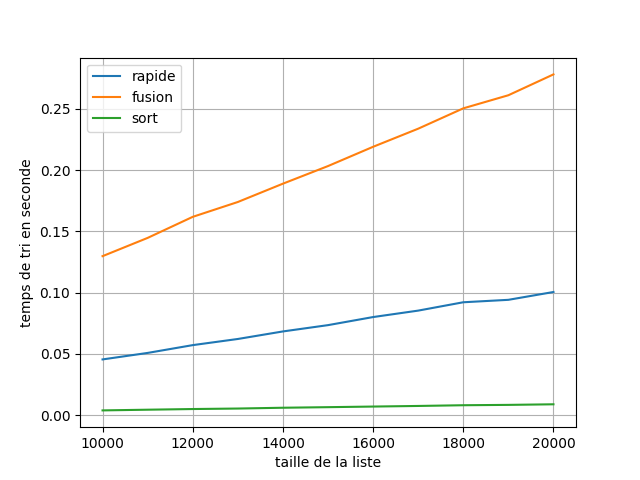
\includegraphics[scale=0.8]{programmes/question_2.png}
\caption{Temps de calcul des tris sans le tri par insertion}
\end{center}
\end{figure}


\question\ Le graphique parle de lui-même.

\question\

\begin{python}
def question_4 () :
    n = 100000
    M = [rd.randint(0,n) for i in range(n)] # liste aléatoire
                                    # de n éléments entre 0 et n
    M.sort() # on trie L

    L = M.copy()                          
    temps=time.time()
    tris.tri_fusion(L,0,n-1)
    temps_fusion = time.time() - temps
            
    L = M.copy() 
    temps=time.time()
    tris.tri_quicksort(L,0,n-1)
    temps_rapide = time.time() - temps
            
    L = M.copy() 
    temps=time.time()
    L.sort()
    temps_sort = time.time() - temps

    return(temps_rapide,temps_fusion,temps_sort)
\end{python}




Le tri rapide n'arrive pas au bout des calculs en un temps raisonnable. Pour le tri fusion, on obtient un temps de 
calcul de $1,53$ secondes, et pour le tri sort, $0,005$ secondes.

\setcounter{question}{0}
\end{corrige}
\else\fi






\section*{Exercice 2 -- Classement de l'étape Tarbes -- La Pierre-Saint-Martin -- 167 km}


\ifprof
\else


Les coureurs du tour de France sont en train de terminer la dixième étape du Tour de France qui sépare Tarbes et La 
Pierre-Saint-Martin. 

Le fichier \texttt{classement\_général} rassemble le classement général à l'issue de l'étape 9. Le fichier \texttt{etape\_10} contient le classement de l'étape 10 uniquement. Dans le fichier texte, les champs sont séparés par des tabulations.


\begin{obj}
L'objectif est de réaliser le classement général après la dixième étape. 
\end{obj}

\subsection*{Lecture des fichiers de résultat}

\setcounter{exo}{0}
\subparagraph{}
\textit{Réaliser la fonction \texttt{charge\_classement} permettant de lire un fichier de classement 
et de retourner une liste de la forme \texttt{[[Nom\_1, Dossard\_1, Temps\_1], [Nom\_2, Dossard\_2, Temps\_2], ...]}. Le temps devra être exprimé en secondes.}



\subsection*{Classement en fin d'étape}
Dans une première approche, on souhaite réaliser le classement général après la fin de l'étape. 

\subparagraph{}
\textit{Réaliser la fonction permettant d'ajouter les temps de l'étape 10 aux temps du classement général.}

\subparagraph{}
\textit{Quel méthode de tri vous semble la mieux adaptée au tri du classement général ?}

\subparagraph{}
\textit{Modifier les algorithmes de tris pour pouvoir trier la liste donnée suivant le temps de course d'un coureur. Le classement général a-t-il changé à l'issue de la dixième étape ?}

\begin{rem}
Travaillant sur une liste de listes, la méthode \texttt{sort} n'est plus adaptée. On peut donc utiliser la fonction, \texttt{sorted} en utilisant une clef de tri (la clef correspondant à la colonne sur laquelle on souhaite trier la liste): 
\end{rem}
\begin{python}
# Tri de la liste <<liste>> sur la colonne 3
sorted(liste, key=lambda colonnes: colonnes[2])
\end{python}



\fi


\ifprof
\begin{corrige}

\question\
\begin{python}
def conversion (temps) :
    """ convertit une chaîne de caractères donnant un temps en
    heures, minutes, secondes, en un nombre de secondes."""
    L = temps.split()
    s = 3600*int(L[0][:len(L[0])-1])+60*int(L[1][:len(L[1])-1])\
    +int(L[2][:len(L[2])-2])
    return s
    
def charge_classement (fichier) :
    f = open(fichier, 'r')
    L = f.readlines()
    f.close()

    classement = []

    for l in L :
        m = l.split('\t')
        classement.append([m[1],m[2],conversion(m[4])])

    return classement
\end{python}

\question\
\begin{python}
def ajout_temps(L1,L2):
    """L1 est la classement de l'étape et L2 le classement général
    certains ont été disqualifiés ou ont abandonné"""
    L=[]
    for dossard in L1:
        L.append(dossard.copy()) # problèmes d'aliasing
        d=dossard[1]
        i=0
        while d != L2[i][1]: #attention certains n'ont pas fait
            # l'étape complètement et sont disqualifiés
            i += 1
        L[-1][-1] += L2[i][-1]
    return L
\end{python}

\question\ Sur des listes de cette taille, peu importe. Tant qu'à faire, autant choisir le tri rapide, ou carrément la 
fonction \texttt{sorted} de python.

\question\ 
\begin{python}
def tri_insertion_modifie(tab):
    """ 
    Trie une liste de nombre en utilisant la méthode du tri par insertion.
    En Python, le passage se faisant par référence, il n'est pas indispensable
    de retourner le tableau.
    Keyword arguments:
    Entrées :
        tab -- liste de nombres
    """
    for i in range (1,len(tab)):
        x=tab[i][-1]
        j=i
        while j>0 and tab[j-1][-1]>x:
            tab[j],tab[j-1]=tab[j-1],tab[j]
            j = j-1
        
    return (tab)
    
td=time.time()
tri_insertion_modifie(ajout_temps(L10,LG))
print('tri insertion des coureurs prend ',time.time()-td,'s')
 

### quicksort modifie
def segmente_modifie(tab,i,j):
    """
    Segmentation d'un tableau par rapport à un pivot.
    Keyword arguments: 
    Entrées :
        tab (list) -- liste de nombres
        i,j (int) -- indices de fin et de début de la segmentation
    Sorties :    
        tab (list) -- liste de nombres avec le pivot à sa place définitive
        k (int) -- indice de la place du pivot
    """
    g =i+1
    d=j
    p=tab[i][-1]
    while g<=d :
        while d>=0 and tab[d][-1]>p:
            d=d-1
        while g<=j and tab[g][-1]<=p:
            g=g+1
        if g<d :
            tab[g],tab[d]=tab[d],tab[g]
            d=d-1
            g=g+1
    k=d
    tab[i],tab[d]=tab[d],tab[i]
    return k
    
def tri_quicksort_modifie(tab,i,j):
    """
    Tri d'une liste par l'utilisation du tri rapide (Quick sort).
    Keyword arguments:
    Entrées :
        tab (list) -- liste de nombres
        i,j (int) -- indices de fin et de début de la zone de tri
    Sorties :    
        tab (list) -- liste de nombres avec le pivot à sa place définitive
    """
    if i<j :
        k = segmente_modifie(tab,i,j)
        tri_quicksort_modifie(tab,i,k-1)
        tri_quicksort_modifie(tab,k+1,j)
        
td=time.time()
tri_quicksort_modifie(ajout_temps(L10,LG),0,len(L10)-1)
print('tri rapide des coureurs prend ',time.time()-td,'s')

### tri fusion modifie
def fusion_listes_modifie(tab,g,d,m):
    """
    Fusionne deux listes triées.
    Keyword arguments:
    Entrées :
        tab (list) -- liste : une liste de nombres tab[g:d] avec g indice de la 
            valeur de gauche, d indice de la valeur de droite
        g,d,m (int) -- entiers : indices tels que g<=m<d et tel que les 
            sous-tableaux tab[g:m] et tab[m+1:d] soient ordonnés
    Sorties :
        tab (list) : liste triée entre les indices g et d
    """
    n1 = m-g+1
    n2 = d-m
    G,D = [],[]
    for i in range (n1):
        G.append(tab[g+i])
    for j in range (n2):
        D.append(tab[m+j+1])
    i,j=0,0
    G.append(['','',99999999999])
    D.append(['','',99999999999])
    for k in range (g,d+1):
        if i<=n1 and  G[i][-1]<=D[j][-1]:
            tab[k]=G[i]
            i=i+1
        elif j<=n2 and G[i][-1]>D[j][-1]:
            tab[k]=D[j]
            j=j+1
            
def tri_fusion_modifie(tab,g,d):
    """
    Tri d'une liste par la méthode du tri fusion
    Keyword arguments:
    Entrées : 
        tab (list) -- liste : une liste de nombres non triés tab[g:d]
        g,d (int) -- entiers : indices de début et de fin de liste si on veut trier
                           tout le tableau g=0, d=len(tab)-1
    Sortie :
        tab (list) : liste triée entre les indices g et d
    """
    if g<d:
        m=(g+d)//2
        tri_fusion_modifie(tab,g,m)
        tri_fusion_modifie(tab,m+1,d)
        fusion_listes_modifie(tab,g,d,m)
        
td=time.time()
tri_fusion_modifie(ajout_temps(L10,LG),0,len(L10)-1)
print('tri fusion des coureurs prend ',time.time()-td,'s')
    

### avec la fonction prédéfinie dans python 'sorted' il faut créer une fonction
### lambda pour travailler sur le 3e élément de chaque élément de la liste

sorted(ajout_temps(L10,LG), key=lambda colonnes: colonnes[2])


td=time.time()
sorted(ajout_temps(L10,LG), key=lambda colonnes: colonnes[2])
print('tri sort python des coureurs prend ',time.time()-td,'s')


# tri insertion des coureurs prend  0.007005929946899414 s
# tri rapide des coureurs prend  0.004002094268798828 s
# tri fusion des coureurs prend  0.004002809524536133 s
# tri sort python des coureurs prend  0.0030019283294677734 s

\end{python}

\setcounter{question}{0}
\end{corrige}
\else\fi


\section*{Exercice 3 -- Tris d'une base de données des films de cinéma}



\ifprof
\else


\setcounter{exo}{0}
\begin{obj}
Réaliser un tri numérique et un tri alphabétique à partir d'une base de données
\end{obj}

On donne le fichier \texttt{films\_martiniere.csv} dans lequel un peu plus de 2000 films sont référencés avec le titre, l'année de création, le réalisateur et le box office.

Une proposition de lecture du fichier csv et de création de la liste de films est donnée ci-dessous et dans le fichier \texttt{lecture\_fichier\_csv.py} :

\begin{python}
f=open('films_martiniere.csv','r')
ligne=f.readline()
fichier=f.readlines()
f.close()

L=[]
for ligne in fichier:
    ligne=ligne.replace('"','')
    ligne=ligne.split(';')
    ligne[-1]=ligne[-1].rstrip('\n')
    ligne[-1]=int(ligne[-1])
    ligne[1]=int(ligne[1])
    L.append(ligne)
\end{python}

Pour ceux qui travaillent avec le logiciel \texttt{Pyzo}, vous devez avoir votre dossier visible dans la fenêtre \texttt{file browser} ou alors exécuter le fichier en cliquant droit sur l'onglet de votre nom de fichier et sélectionner \textit{Exécuter en tant que script}. Votre fichier python et le fichier \texttt{films\_martiniere.csv} doivent être dans le même dossier.

\subparagraph{}
\textit{Commenter chaque ligne du programme proposé de lecture du fichier csv. %Copier vos tests dans le script python.
}

\subparagraph{}
\textit{A partir de l'étude réalisée dans l'exercice 2, choisir l'algorithme de tri le plus efficace pour trier le 
fichier de 2000 films. Copier l'algorithme choisi dans votre script et le modifier afin qu'il puisse trier une liste 
de listes.}

\subparagraph{}
\textit{Trier les films en fonction du box office. Quel est le film qui a été le plus vu au cinéma ?}

% \subparagraph{}
% \textit{Définir la fonction \texttt{comparer} qui a pour argument une liste de deux mots \texttt{mot1} et 
% \texttt{mot2} et qui renvoie cette liste triée par ordre alphabétique. Les mots de la liste seront écrits en lettres 
% majuscules. Les titres de films peuvent comporter des chiffres.}

\subparagraph{}
\textit{Implémenter un algorithme de tri alphabétique adapté au fichier de films. Les titres de films sont écrits en 
lettres majuscules et peuvent comporter des chiffres et des caractères spéciaux. Quel est le titre du premier film de 
la liste ?}



\fi


\ifprof
\begin{corrige}

\question\
\begin{python}
f=open('films_martiniere.csv','r')
ligne1=f.readline() # on élimine la première ligne
fichier=f.readlines()
f.close()

L=[]
for ligne in fichier:
    ligne=ligne.replace('"','') # enlever les guillemets
    ligne=ligne.split(';') # création d'une liste en coupant au niveau des ;
    ligne[-1]=ligne[-1].rstrip('\n')
    ligne[-1]=int(ligne[-1]) # remplacer la chaine de caractères par un entier
    ligne[1]=int(ligne[1]) # remplacer la chaine de caractères par un entier
    L.append(ligne)
\end{python}

\question\ On utilisera la fonction \texttt{sorted}.

\question\ 
\begin{python}
M = sorted(L, key = lambda colonnes : colonnes[-1], reverse = True)
\end{python}

Il suffit de demander \texttt{M[0]}, et l'on obtient \texttt{['INTOUCHABLES', 2011, 'ERIC TOLEDANO', 35648468]}.

\question\ Les commandes \texttt{python} $<$, $>$, $\leqslant$ et $geqslant$ permettant tout à fait de comparer des 
chaînes de caractère, même avec des caractères spéciaux, nous pouvons utiliser directement le tri 
\texttt{tri_quicksort_modifie}.

\begin{python}
def segmente_modifie_bis(tab,i,j):
    """
    Segmentation d'un tableau par rapport à un pivot.
    Keyword arguments: 
    Entrées :
        tab (list) -- liste de nombres
        i,j (int) -- indices de fin et de début de la segmentation
    Sorties :    
        tab (list) -- liste de nombres avec le pivot à sa place définitive
        k (int) -- indice de la place du pivot
    """
    g =i+1
    d=j
    p=tab[i][0]
    while g<=d :
        while d>=0 and tab[d][0]>p:
            d=d-1
        while g<=j and tab[g][0]<=p:
            g=g+1
        if g<d :
            tab[g],tab[d]=tab[d],tab[g]
            d=d-1
            g=g+1
    k=d
    tab[i],tab[d]=tab[d],tab[i]
    return k
    
def tri_quicksort_modifie_bis(tab,i,j):
    """
    Tri d'une liste par l'utilisation du tri rapide (Quick sort).
    Keyword arguments:
    Entrées :
        tab (list) -- liste de nombres
        i,j (int) -- indices de fin et de début de la zone de tri
    Sorties :    
        tab (list) -- liste de nombres avec le pivot à sa place définitive
    """
    if i<j :
        k = segmente_modifie_bis(tab,i,j)
        tri_quicksort_modifie_bis(tab,i,k-1)
        tri_quicksort_modifie_bis(tab,k+1,j)

N = tri_quicksort_modifie_bis(L,0,len(L)-1)
\end{python}

Il suffit de demander \texttt{N[0]}, et l'on obtient \texttt{["'71", 2014, 'YANN DEMANGE', 133694]}.

\setcounter{question}{0}
\end{corrige}
\else\fi